%
% Modified by Megan Patnott
% Last Change: Jan 18, 2013
%
%%%%%%%%%%%%%%%%%%%%%%%%%%%%%%%%%%%%%%%%%%%%%%%%%%%%%%%%%%%%%%%%%%%%%%%%
%
% Modified by Sameer Vijay
% Last Change: Tue Jul 26 2005 13:00 CEST
%
%%%%%%%%%%%%%%%%%%%%%%%%%%%%%%%%%%%%%%%%%%%%%%%%%%%%%%%%%%%%%%%%%%%%%%%%
%
% Sample Notre Dame Thesis/Dissertation
% Using Donald Peterson's ndthesis classfile
%
% Written by Jeff Squyres and Don Peterson
%
% Provided by the Information Technology Committee of
%   the Graduate Student Union
%   http://www.gsu.nd.edu/
%
% Nothing in this document is serious except the format.  :-)
%
% If you have any suggestions, comments, questions, please send e-mail
% to: ndthesis@gsu.nd.edu
%
%%%%%%%%%%%%%%%%%%%%%%%%%%%%%%%%%%%%%%%%%%%%%%%%%%%%%%%%%%%%%%%%%%%%%%%%


%
% Chapter 1
%

\chapter{Introduction}

\section{Overview}

This is an overview of the introduction.  In here, I will use many
many buzzwords and other legalistic-types of terms, mostly beginning on
the expounding of the holistic and synergistic energy that Gnus bring
to our organizations.

\subsection{Background}

In preparation for reading this dissertation, I would highly recommend
reading some of the other material available on
Gnus~\citep{gnus98:_gerry_ganst,greenfield96:_gettin_know_gnu}.  They
are very well written and will give you a fuller understanding of
Gnus.

Gnus are frequently mistakes for squirrels.  They are not squirrels.
They are Gnus.  Don't call them squirrels, either (unless you have
food in your hand); they tend to get a bit upset.\footnote{This is
  frequently mistaken for the chattering and scampering away.  Gnus
  are actually quite polite; they will leave if they have nothing nice
  to say, for fear of saying something offensive.}  If you have food
in your hand, they tend to ignore this insult and accept your food as
a peace offering.\footnote{Sometimes they'll follow you if you continue
to refuse to feed them.}

\subsection{Foreground}

Table~\ref{tbl:bogus1} shows some feeding frequencies for where Gnus
like to eat around the Notre Dame campus.  Gnus have work weeks, just
like humans do, hence the much lower frequencies on weekends.  This
can lead us to conclude that Gnu weekend shifts are much smaller than
the normal work-week shifts.  In fact, we can attempt to parametrize the
sighting frequency, $\mathcal{F}$, by the student population, type of food, and
day of the week as:
\begin{equation}
  \mathcal{F} = \mathcal{F}(p,f,d).
\end{equation}
Table~\ref{tbl:bogus2} shows what they
typically like to eat.

\begin{table}[tpb]
  \begin{center}
    \caption{Where \NoCaseChange{Gnus} Like to eat \label{tbl:bogus1}}
    \begin{tabularx}{0.85\textwidth}{lrrrrrrr} \toprule
      \multicolumn{1}{c}{Location} & Sun & Mon & Tue & Wed & Thu & Fri & Sat \\ \midrule
      Front of Dome & 1 & 5 & 6 & 5 & 4 & 5 & 1 \\
      Stonehenge & 2 & 9 & 10 & 12 & 9 & 14 & 2 \\
      The Rock & 1 & 3 & 4 & 3 & 4 & 3 & 0 \\
      The ACC & 3 & 4 & 5 & 5 & 5 & 4 & 1 \\
      Dining Halls & 5 & 14 & 12 & 13 & 14 & 12 & 3 \\
      Hesburgh Library & 2 & 3 & 5 & 2 & 3 & 4 & 2 \\ \bottomrule
    \end{tabularx}
  \end{center}
\end{table}

\begin{table}[tpb]
  \setlength{\capwidth}{0.7\textwidth}
  \begin{center}
    \caption{What \NoCaseChange{Gnus} like to eat on the Notre Dame Campus, Listed
      by Average Number of Sightings per Weekday
    \label{tbl:bogus2}
}
    \begin{tabular}{lrrrrrrr} \toprule
      \multicolumn{1}{c}{Food} & Sun & Mon & Tue & Wed & Thu & Fri & Sat \\ \midrule
      Twinkies & 1 & 5 & 6 & 5 & 4 & 5 & 1 \\
      Ding Dongs & 2 & 9 & 10 & 12 & 9 & 14 & 2 \\
      Carrots & 1 & 3 & 4 & 3 & 4 & 3 & 0 \\
      Lettuce & 3 & 4 & 5 & 5 & 5 & 4 & 1 \\
      Twizlers & 5 & 14 & 12 & 13 & 14 & 12 & 3 \\
      Jawbreakers & 2 & 3 & 5 & 2 & 3 & 4 & 2 \\ \bottomrule
    \end{tabular}
  \end{center}
\end{table}

Figure~\ref{fig:bogus3} shows a nice graph of location distributions
by day of week.  I have no real reason for including it except to show
that figures work as well.  Did I mention that Gnus are really cool?

\begin{figure}[tpb]
  \begin{center}
    \centerline{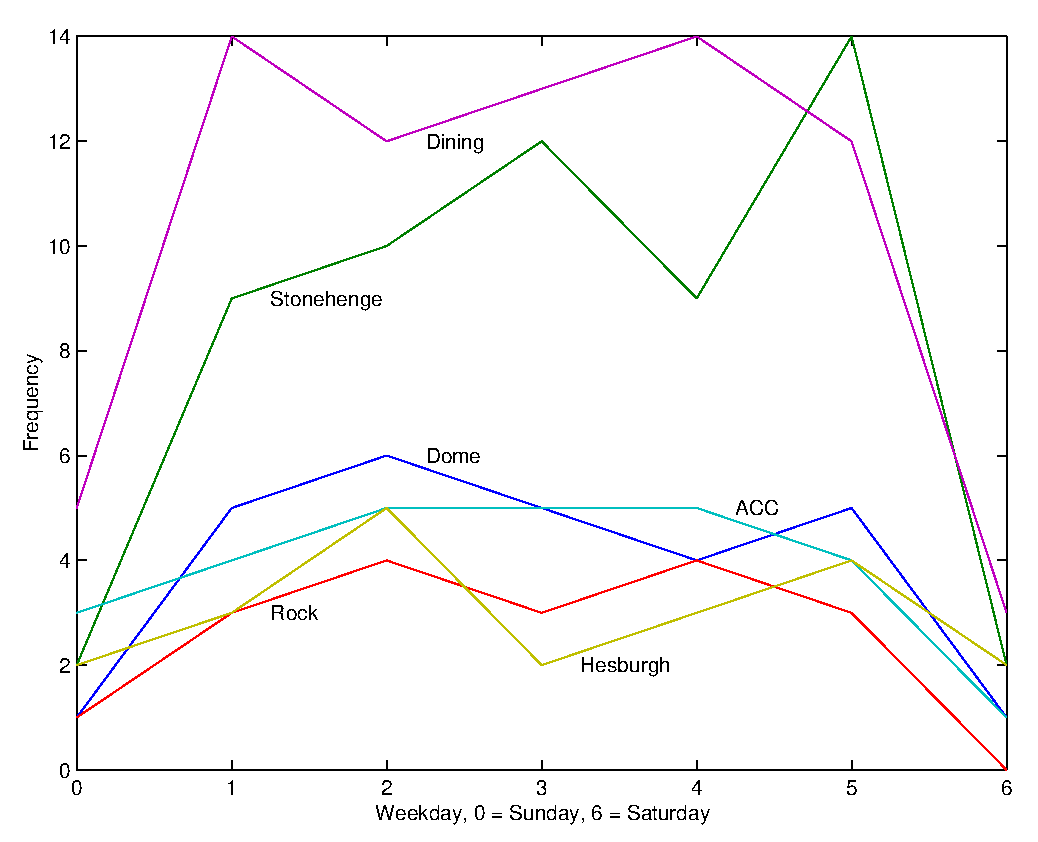
\includegraphics[scale=0.8]{sample_nd}}
    \caption{Location distributions by day of where, where the X axis
      is the weekday (0 through 6), and the Y axis is the sighting
      frequency}
    \label{fig:bogus3}
  \end{center}
\end{figure}

Gnus typically tend to come out when there are large gatherings of
humans with food.  Gnus work very hard at providing us with all the
things that we like (trees, dirt, air, etc.), and so we should freely
give them food.  They will come up and stand a respectful distance
away from you, waiting to see if they will be rewarded for their
efforts.  If you offer some food, they will take it and back off a
respectful distance in order to consume their food while leaving you
to your ``personal space.''  

\section{Groovin' Gnus}
\label{sec:groovin-gnus}

Gnus do tend to stay away from humans in their normal day-to-day
workings.  This is mainly because humans don't, for the most part,
understand what they are doing.  If a Gnu is working, and a human
approaches it, the Gnu will tend to drop whatever it is doing and run
away.  This is probably do to the tendency for humans to have ``group
meetings'' and ``productivity seminars.''  Most Gnus are deathly
afraid of such overmanagement, and run at the slightest hint of it,
for fear that it will cripple their real work.

It is interesting, however, that Gnus have chosen an Institution of
Higher Education for their BOO.\footnote{Base of Operations.}  It is
often said that:
\begin{quote}
  Academic politics are the dirtiest, meanest, ugliest, and generally
  the most low-down, in-your-face, and kick-em-while-they're-down than
  anywhere else (even Washington D.C.)  because the stakes are so low.
\end{quote}
It has been hypothesized that the Gnus are subtly trying to affect a
change for the better (i.e., eliminating the overmanagement problems)
by working the very system that they are trying to change, from
within.  That is, the graduates from Notre Dame can learn from the
examples of the Gnus here, and run screaming (or chattering) at the
slightest hint of overmanagement, and let the real work proceed
unhindered.

% % uncomment the following lines,
% if using chapter-wise bibliography
%
% \bibliographystyle{ndnatbib}
% \bibliography{example}
